  \section[Nationwide Health Information Network (NwHIN)]{NwHIN}
  \label{sec:nwhin}

  \initial{N}\textit{ationwide Health Information Network (NwHIN )}\
  is a set of standards, services, and policies that enable the secure exchange\
  of health information over the Internet.\citep{_nwhin_framework_2013}
 This is currently achieved through three different initiatives:\
  \begin{itemize}
    \itemsep0ex
    \item  NwHIN Exchange
    \item  NwHIN Direct 
    \item Aurion Software
  \end{itemize}

  \subsection{NwHIN Exchange}

 	NwHIN Exchange is a more complex exchange protocol that has methods\
to perform universal patient lookup, document discovery and retrieval,\
 and exchange between organizations and federal agencies\
 (VA, DOD, CDC, SSA, plus 22 others). The organizations entering into\
 an exchange with those federal agencies are typically sizable HIOs, HIEs\
or large IDNs. Participation in the NwHIN Exchange is currently limited to\
federal health agencies and healthcare organizations under ONC contract\
 and other recipients of federal grants. There are technical teams devoted\
 to the on-boarding process (validation and conformance testing), security,\
 authentication, and adherence to the specifications standards, including\
 producing/accepting structured data in defined formats.\
\citep{_nwhin_exchange_2013}\\

  	Most individual providers/small practices don't have the technical capability\
 to implement this exchange. That's where the other initiatives such as the\
NwHIN Direct and the Aurion Software come into play to allow for a more\
 simpler path to achieving the goals of the program.\\

 \subsection{NwHIN Direct}

 	NwHIN Direct known as a simpler alternative to NwHin Exchange\
also enables standards-based health information exchange in support\
 of core Stage 1 MU measures, including communication of summary\
care records, referrals, discharge summaries and other clinical documents in\
 support of continuity of care and medication reconciliation, and communication\
 of laboratory results to providers. It exclusively supports cases of\
 “pushed communication” between providers, hospitals and laboratories.\
 It also consists of Authentication, certificates, vocabulary messaging standards and security.\\

The key difference between Exchange and Direct is messaging:\
 the NwHIN Direct specifications will support unstructured messages\
(i.e., simple text or PDF), semi-structured text, and highly structured messages\
 like CCD C32. NwHIN Direct is not currently capable of supporting MU exchange\
requirements beyond elemental Stage 1 requirements.\
\citep{_nwhin_exchange_2013}\

 \begin{figure}[ht!]
    \centering
    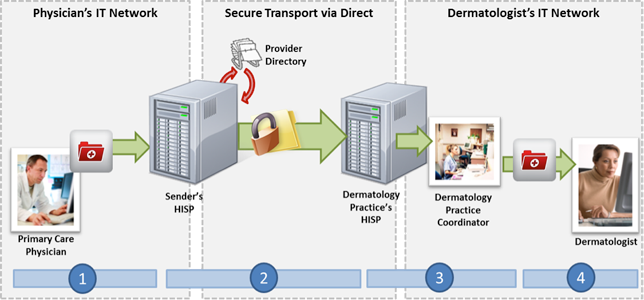
\includegraphics[scale=0.5]{nwhin.png}
    \caption{Transferring of Patient Record from one provider to another using DIRECT}
    \cite[Fig.~1]{_nwhin_frameworkOne_2013}
    \label{fig:nwhin}
  \end{figure}  

  \subsection{Aurion Software}

	Formally known as CONNECT, Aurion is an open source health information\
exchange platform that implements the Nationwide Health Information Network\
 standard services and content specifications. This software enables the\
secure exchange of interoperable health information among diverse organizations\
 using a wide variety of technologies.\\

By implementing Aurion, organizations as a part of their health information\
 exchange strategy gain the benefits of implementing nationally-recognized\
 standards enabling data exchange with federal agencies as well as with numerous\
 other health IT stakeholders. Aurion enables health professionals to request,\
 send and receive medical records so critical information can follow patients\
as they navigate through the health care system. The software places relevant\
 patient medical data at the doctor’s fingertips. It enhances security, promotes\
 public health, and empowers patients to be more active and involved in their\
 own care decisions.\citep{_aurion_software_2013}
